%% Author_tex.tex
%% V1.0
%% 2012/13/12
%% developed by Techset
%%
%% This file describes the coding for rsproca.cls

\documentclass[]{rsos}%%%%where rsos is the template name


\usepackage[T1]{fontenc}
\usepackage[utf8]{inputenc}

% Pandoc citation processing


%%%% *** Do not adjust lengths that control margins, column widths, etc. ***

%%%%%%%%%%% Defining Enunciations  %%%%%%%%%%%
\newtheorem{theorem}{\bf Theorem}[section]
\newtheorem{condition}{\bf Condition}[section]
\newtheorem{corollary}{\bf Corollary}[section]
%%%%%%%%%%%%%%%%%%%%%%%%%%%%%%%%%%%%%%%%%%%%%%%

\begin{document}

%%%% Article title to be placed here
\title{Template for preparing your research report submission to Royal Society Open Science using RMarkdown}

\author{
Alice Anonymous$^{1,2}$,
Bob Security$^{2}$}

\address{
  $^{1}$Some Institute of Technology, Department, Street, City, State, Zip\\
  $^{2}$Another University Department, Street, City, State, Zip}
%%%% Subject entries to be placed here %%%%
\subject{
subject 1,
subject 2,
subject 3}

%%%% Keyword entries to be placed here %%%%
\keywords{
one,
two,
optional,
optional,
optional}

%%%% Insert corresponding author and its email address}
\corres{
  B. Security\\
  e-mail: \href{mailto:bob@email.com}{\nolinkurl{bob@email.com}}
}

%%%% Abstract text to be placed here %%%%%%%%%%%%
\begin{abstract}
The abstract text goes here. The abstract text goes here. The abstract text goes here. The abstract text goes here. The abstract text goes here. The abstract text goes here. The abstract text goes here. The abstract text goes here.
\end{abstract}
%%%%%%%%%%%%%%%%%%%%%%%%%%%

%% Some pieces required from the pandoc template
\providecommand{\tightlist}{%
  \setlength{\itemsep}{0pt}\setlength{\parskip}{0pt}}
\providecommand{\EndFirstPage}{%
}

\begin{fmtext}

\hypertarget{insert-a-head-here}{%
\section{Insert A head here}\label{insert-a-head-here}}

This demo file is intended to serve as a ``starter file''" for articles submitted to the \href{http://rsos.royalsocietypublishing.org/}{Royal Society Open Science} journal using \texttt{RMarkdown}.

Place \texttt{\textbackslash{}EndFirstPage} at the point where the plain text on the first page stops. Warning: excess text will be hidden behind the copyright box. The example below contains line 1 to 19 in the code. Lines 14 to 17 are hidden behind the copyright box.

\hypertarget{insert-b-head-here}{%
\subsection{Insert B head here}\label{insert-b-head-here}}

Subsection text here.

\hypertarget{insert-c-head-here}{%
\subsubsection{Insert C head here}\label{insert-c-head-here}}

Subsubsection text here.

Line 1

Line 2

Line 3

Line 4

Line 5

Line 6

Line 7

Line 8

Line 9

Line 10

Line 11

Line 12

Line 13

Line 14

Line 15

Line 16

Line 17

Line 18

Line 19

\end{fmtext}
\maketitle

\hypertarget{lists}{%
\section{Lists}\label{lists}}

\begin{itemize}
\item
  one
\item
  two
\item
  three
\item
  fruits

  \begin{itemize}
  \tightlist
  \item
    apples

    \begin{itemize}
    \tightlist
    \item
      macintosh
    \item
      red delicious
    \end{itemize}
  \item
    pears
  \item
    peaches
  \end{itemize}
\item
  vegetables

  \begin{itemize}
  \tightlist
  \item
    broccoli
  \item
    chard
  \end{itemize}
\end{itemize}

\hypertarget{citations}{%
\subsection{Citations}\label{citations}}

Blabla \cite{Lannes} blabla. Blabla \cite{HJ2} blabla. Blabla \cite{BF, Lannes} blabla. Blabla \cite{Benjamin1967, HJ2, HJ3, HP2} blabla.

\hypertarget{headling-level-3}{%
\subsubsection{Headling level 3}\label{headling-level-3}}

Subsubsection text here.

\hypertarget{r-code}{%
\section{R code}\label{r-code}}

R code can be added as usual. Note that syntax highlighting is not available. Fig. \ref{fig:nice-plot} is a an example.

\begin{verbatim}
#23456789012345678901234567890123456789012345678901234567890123456789012345
#       10        20        30        40        50        60        70     
summary(lm(mpg ~ disp, data = mtcars))
\end{verbatim}

\begin{verbatim}
## 
## Call:
## lm(formula = mpg ~ disp, data = mtcars)
## 
## Residuals:
##     Min      1Q  Median      3Q     Max 
## -4.8922 -2.2022 -0.9631  1.6272  7.2305 
## 
## Coefficients:
##              Estimate Std. Error t value Pr(>|t|)    
## (Intercept) 29.599855   1.229720  24.070  < 2e-16 ***
## disp        -0.041215   0.004712  -8.747 9.38e-10 ***
## ---
## Signif. codes:  0 '***' 0.001 '**' 0.01 '*' 0.05 '.' 0.1 ' ' 1
## 
## Residual standard error: 3.251 on 30 degrees of freedom
## Multiple R-squared:  0.7183, Adjusted R-squared:  0.709 
## F-statistic: 76.51 on 1 and 30 DF,  p-value: 9.38e-10
\end{verbatim}

\begin{verbatim}
##       mpg             cyl             disp             hp       
##  Min.   :10.40   Min.   :4.000   Min.   : 71.1   Min.   : 52.0  
##  1st Qu.:15.43   1st Qu.:4.000   1st Qu.:120.8   1st Qu.: 96.5  
##  Median :19.20   Median :6.000   Median :196.3   Median :123.0  
##  Mean   :20.09   Mean   :6.188   Mean   :230.7   Mean   :146.7  
##  3rd Qu.:22.80   3rd Qu.:8.000   3rd Qu.:326.0   3rd Qu.:180.0  
##  Max.   :33.90   Max.   :8.000   Max.   :472.0   Max.   :335.0  
##       drat             wt             qsec             vs        
##  Min.   :2.760   Min.   :1.513   Min.   :14.50   Min.   :0.0000  
##  1st Qu.:3.080   1st Qu.:2.581   1st Qu.:16.89   1st Qu.:0.0000  
##  Median :3.695   Median :3.325   Median :17.71   Median :0.0000  
##  Mean   :3.597   Mean   :3.217   Mean   :17.85   Mean   :0.4375  
##  3rd Qu.:3.920   3rd Qu.:3.610   3rd Qu.:18.90   3rd Qu.:1.0000  
##  Max.   :4.930   Max.   :5.424   Max.   :22.90   Max.   :1.0000  
##        am              gear            carb      
##  Min.   :0.0000   Min.   :3.000   Min.   :1.000  
##  1st Qu.:0.0000   1st Qu.:3.000   1st Qu.:2.000  
##  Median :0.0000   Median :4.000   Median :2.000  
##  Mean   :0.4062   Mean   :3.688   Mean   :2.812  
##  3rd Qu.:1.0000   3rd Qu.:4.000   3rd Qu.:4.000  
##  Max.   :1.0000   Max.   :5.000   Max.   :8.000
\end{verbatim}

\begin{figure}

{\centering 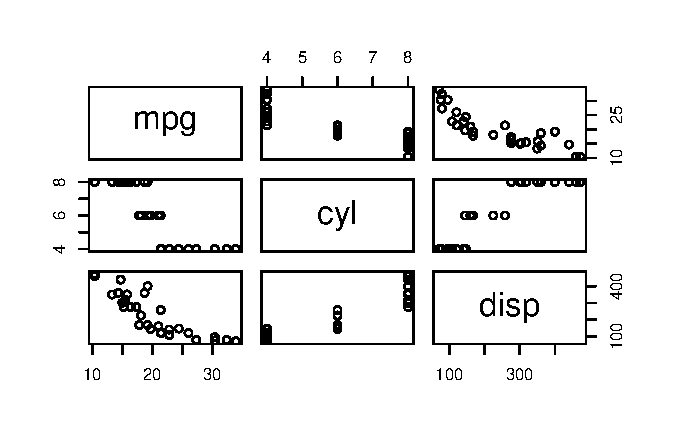
\includegraphics{RSOSJA_files/figure-latex/nice-plot-1} 

}

\caption{The caption}\label{fig:nice-plot}
\end{figure}

\ethics{Please provide details on the ethics.}

\dataccess{Please provide details on the data availability.}

\aucontribute{Please provide details of author contributions here.}

\competing{Please declare any conflict of interest here.}

\funding{Please provide details on funding}

\disclaimer{Please provide disclaimer text here.}

\ack{Please include your acknowledgments here, set in a single paragraph. Please do not include any acknowledgments in the Supporting Information, or anywhere else in the manuscript.}

\bibliographystyle{RS}
\bibliography{sample.bib}


\end{document}
